\documentclass[10pt]{article}
\usepackage[a4paper,margin=2.4cm]{geometry}
\usepackage{amsmath,amssymb}
\usepackage{booktabs}
\usepackage{graphicx}
\usepackage{microtype}
\usepackage[hidelinks]{hyperref}
\usepackage{caption}
\captionsetup{font=small,labelfont=bf}

\newcommand{\blkstep}{\mathrm{blk/step}}

\title{Sparse Goal Edits and Variable-Duration Options\\in World-Model Hierarchical RL}
\author{George Vasilache}
\date{Working draft --- \today}

\begin{document}
\maketitle

\begin{abstract}
We study two restrictions on the manager of a Director-style hierarchical agent
built on DreamerV3: (i) \emph{masked goal edits}, where the manager maintains a
persistent goal code and edits only a sparse subset of its blocks per decision,
and (ii) \emph{variable decision durations}, where the manager chooses how long
each goal is held. Both are motivated by decision sparsity: fewer and more local
manager interventions per environment step. On dense-reward cartpole the combined
recipe outperforms each component alone and reaches returns of $\sim$840,
competitive with the best fixed-schedule variants; on cheetah, replacing fixed
sparsity/duration targets with Lagrangian controllers roughly doubles the return.
On sparse-reward tasks (hopper hop, acrobot swingup) every variant tested so far
fails to encounter reward, while the unrestricted Director baseline learns.
A controlled comparison isolates the variable-duration mechanism at short target
durations as sufficient for this failure, and ongoing experiments test whether
duration targets, duration--return coupling, or goal-edit locality is responsible.
\end{abstract}

\section{Setting}
\label{sec:setting}

The base agent is a reimplementation of Director-style hierarchy on DreamerV3.
A recurrent state-space world model provides latent states $s_t$. A goal
autoencoder discretizes latent goals: an encoder maps a target state to a code
$z \in \{1,\dots,C\}^{L}$ of $L$ categorical blocks ($L{=}8$ on the tasks used
here), and a decoder maps codes back to latent goals. A \emph{manager} policy
selects codes every $K$ steps (Director: fixed $K{=}8$) and is trained on
extrinsic plus exploration reward; a \emph{worker} policy receives the decoded
goal and is trained on a goal-reaching reward. All training happens in
imagination; the worker never observes task reward directly.

We investigate whether manager decisions can be made \emph{sparser} without
loss of control performance, along two axes:

\textbf{Masked goal edits.} The manager maintains a running goal code $Z_t$ and
at each decision outputs a new code $z_t$ together with a binary mask
$m_t \in \{0,1\}^{L}$, updating
\begin{equation}
Z_{t} \;=\; m_t \odot z_t \;+\; (1-m_t)\odot Z_{t-1},
\label{eq:edit}
\end{equation}
so only the selected blocks change and the rest of the goal persists.

\textbf{Variable durations.} Alongside the goal, the manager outputs a hold
duration $d_t \in \{1,\dots,16\}$; the next decision occurs after $d_t$ steps
rather than on a fixed schedule.

The natural cost measure combining both axes is the average number of goal
blocks edited per environment step,
\begin{equation}
\blkstep \;=\; \frac{\mathbb{E}[\|m\|_1]}{\mathbb{E}[d]}
       \;=\; \frac{\bar{m}\,L}{\bar{K}},
\label{eq:blkstep}
\end{equation}
where $\bar m$ is the mean edit fraction and $\bar K$ the realized mean
duration. Director corresponds to $\bar m{=}1$, $\bar K{=}8$, i.e.\
$\blkstep = 1$.

\paragraph{Motivation.} If performance can be held while $\blkstep$ drops well
below 1, manager decisions become temporally extended \emph{and} spatially
local: the goal stream turns into a piecewise-constant program with sparse
diffs. Anticipated benefits are (a) interpretability---individual block edits
can be attributed to behavior changes; (b) a controllable knob for temporal
abstraction; (c) less non-stationarity in the worker's objective, since most of
the goal persists across decisions.

\section{Sparsity and duration control}
\label{sec:method}

Direct penalties on edit fraction or duration proved brittle (Sec.~\ref{sec:results});
the current recipe controls both with dual-ascent Lagrangian controllers of the
same form. For a statistic $x$ (e.g.\ mean mask probability) with target
$\tau$, a multiplier $\lambda$ is updated toward satisfying the constraint and
the term $\lambda\,x$ is added to the manager loss:
\begin{equation}
\lambda \leftarrow \operatorname{clip}\!\big(\lambda \cdot \exp(\eta\,(x - \tau)),\;
\lambda_{\min},\, \lambda_{\max}\big).
\label{eq:dual}
\end{equation}

Three such controllers are active in the combined (``group D'') recipe:
\begin{itemize}\itemsep2pt
\item \textbf{Edit-rate}: mean mask probability $\to$ target $0.3$
  (mode \texttt{prob}).
\item \textbf{Per-block entropy}: mean per-block mask entropy $\to$ target
  $0.5$, preventing collapse onto always/never-edited blocks
  (mode \texttt{entropy}; \texttt{prob\_entropy} runs both).
\item \textbf{Duration}: the switch-weighted deviation
  $|\mathbb{E}[d]-\tau_d|$ $\to$ tolerance $0.1$, with $\tau_d \in \{4,8\}$.
  Regulating the deviation (rather than raw duration) keeps the controller
  symmetric; it relaxes to $\lambda\!\to\!0$ once within tolerance.
\end{itemize}

Additionally, a \emph{structural consistency} loss with weight $w_s$ (default
200) ties code-space distances to latent state distances, so that small code
edits correspond to nearby goals:
\begin{equation}
\mathcal{L}_{\text{struct}} =
\big\| \mathrm{dist}(z_i, z_j) - \mathrm{dist}(s_i, s_j) \big\|^2 ,
\qquad \text{realized corr.} \approx 0.92\text{--}0.98 .
\label{eq:struct}
\end{equation}

The manager's per-decision reward aggregates the extrinsic reward over the held
segment with a \emph{mean} by default,
$r^{\text{mgr}}_i = \frac{1}{d_i}\sum_{t \in \text{seg}_i} r_t$,
which makes the manager's return invariant to how finely time is partitioned;
a \emph{sum} aggregation ($r^{\text{mgr}}_i = \sum_{t\in\text{seg}_i} r_t$,
Director-style) couples return to duration and is under test
(Sec.~\ref{sec:ongoing}).

\section{Experimental setup}

Tasks are DeepMind Control from pixels (+proprio): cartpole swingup and cheetah
run (dense reward), hopper hop and acrobot swingup (sparse/impulsive reward).
Two scales are used (Table~\ref{tab:scales}); all runs are 4M environment
steps, seed 0, on the Saion cluster. Experiments are numbered globally
(\texttt{e}$n$) and logged in \texttt{EXPERIMENTS.md}; scores below are means
over the last 10 episodes (``last10'') and the best trailing-10 window
(``peak'').

\begin{table}[h]
\centering\small
\begin{tabular}{lllll}
\toprule
Scale & Image & Model & Batch & Hardware \\
\midrule
small & $32^2$ & size6m & $16\times32$ & 1$\times$V100 \\
BIG (\texttt{director\_match}) & $64^2$ & deter 1024, 512-wide MLPs & $16\times64$ & 1$\times$A100-80GB \\
\bottomrule
\end{tabular}
\caption{Run scales. BIG matches the published Director architecture.}
\label{tab:scales}
\end{table}

\section{Results to date}
\label{sec:results}

\begin{table}[h]
\centering\small
\begin{tabular}{llrrl}
\toprule
Task & Recipe (BIG scale) & last10 & peak & Reference \\
\midrule
cartpole & combined mask+var-$K$+struct (D) & 776 & 844 & e171 (e157: 833/869) \\
cartpole & mask only, fixed $K{=}8$        & 360 & 419 & e163 (history: e9 $\approx$ 1) \\
cartpole & var-$K$ only, target 4          &  97 & 658 & e167 (collapsed) \\
cartpole & plain var-$K$ + struct, target 8 & 725 & 758 & e46 (small scale) \\
cheetah  & combined, Lagrangian controllers & 465 & 508 & e175 \\
cheetah  & combined, fixed targets          & 253 & --  & e142 \\
hopper   & \emph{any} masked / var-$K$ variant & 0 & $\sim$6 & e164--e173 (all) \\
hopper   & Director baseline, fixed $K{=}8$ & $\sim$300 & -- & e124 \\
acrobot  & combined (D), targets 4          & $\sim$1 & 37 & e176/e177 \\
\bottomrule
\end{tabular}
\caption{Key results. Returns are episode scores (max 1000).}
\label{tab:results}
\end{table}

\begin{figure}[t]
\centering
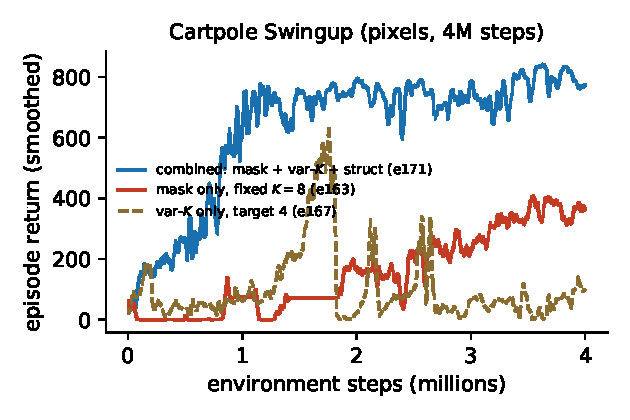
\includegraphics[width=.48\linewidth]{figures/cartpole_components.pdf}\hfill
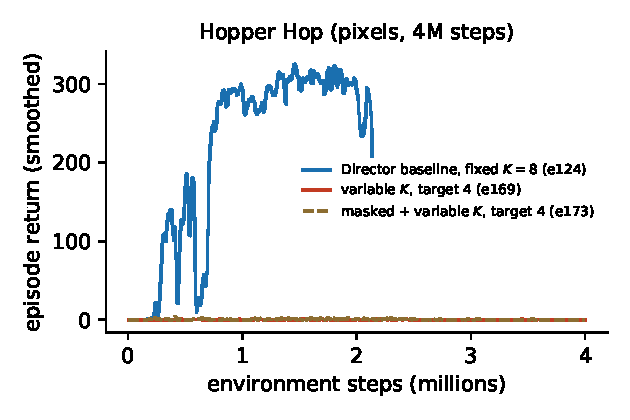
\includegraphics[width=.48\linewidth]{figures/hopper_vark.pdf}
\caption{Left: on cartpole the combined recipe (mask + variable $K$ + struct)
clearly outperforms either component alone. Right: on hopper the Director
baseline (fixed $K{=}8$, full goal replacement) learns, while the
variable-duration variant with target 4 --- differing \emph{only} in the
variable-duration package --- never encounters reward; adding masking does not
change this.}
\label{fig:curves}
\end{figure}

\paragraph{1. The components interact; neither suffices alone.}
On cartpole, masked edits at fixed $K{=}8$ and variable $K$ without
masking/struct both underperform the combined recipe by a large margin
(Table~\ref{tab:results}, Fig.~\ref{fig:curves} left). This is consistent
across the program's history: masked fixed-$K{=}8$ variants collapsed or
plateaued (best 511), and plain variable-$K$ needed both a duration prior and
the structural loss to reach 724. The combined recipe achieves
$\blkstep \approx 0.6$--$1.1$ at returns of 776--844, versus Director's
$\blkstep = 1$.

\paragraph{2. Lagrangian controllers transfer better than fixed penalties.}
Replacing fixed sparsity/duration penalty weights with the controllers of
Eq.~\eqref{eq:dual} left cartpole unchanged but roughly doubled cheetah
(253 $\to$ 465--508), the best cheetah result in the program. The duration
controller behaves as intended: the multiplier relaxes to 0 once
$|\mathbb{E}[d]-\tau_d|$ is within tolerance, and the realized duration stays
at the target without an active constraint.

\paragraph{3. Sparse-reward tasks fail under every restricted variant.}
On hopper, every masked and/or variable-duration configuration tested (16+
runs across recipes, scales, and controller variants) shows manager extrinsic
reward $\approx 10^{-4}$ throughout training --- the reward is never
encountered, so nothing downstream can learn. The Director baseline (e124)
finds reward within 0.2--0.4M steps and reaches $\sim$300. Acrobot behaves
like hopper under the combined recipe.

\paragraph{4. A controlled comparison implicates short variable durations.}
Resolved-configuration diffs show e169 (variable $K$, duration target 4, no
mask, no struct) and e124 (fixed $K{=}8$) differ \emph{only} in the
variable-duration package (Fig.~\ref{fig:curves} right). Two mechanisms could
explain the failure: (i) \emph{commitment} --- re-deciding every $\sim$4 steps
may not persist long enough with one goal to leave the low-reward region;
(ii) \emph{duration--return decoupling} --- with mean aggregation
(Sec.~\ref{sec:method}) the manager has no return incentive to hold longer.
Goal-edit \emph{locality} (mask + struct + persistent goal restricting how far
the proposed goal can move per decision) remains a candidate for the masked
variants, which fail on hopper even at fixed $K{=}8$ with high worker action
entropy.

\section{Ongoing experiments}
\label{sec:ongoing}

Seven runs launched 2026-07-13 (all BIG, 4M steps) separate these hypotheses.
Early signals at $\sim$0.12M steps are annotated; the ``alive'' criterion is
reward rate $>10^{-2}$ by 1M steps (e124 reference).

\begin{table}[h]
\centering\small
\begin{tabular}{lllll}
\toprule
Exp & Configuration & Task & Tests & Early signal \\
\midrule
e178 & var-$K$, target 8 (e169 + one knob) & hopper & commitment (i) & reward rate $1.5{\times}10^{-3}$ \\
e179 & var-$K$, target 8 & cartpole & does struct matter at $\tau_d{=}8$? & learning (141 @ 0.12M) \\
e180 & Director baseline & acrobot & is acrobot hard for the base? & \emph{learning} (0.13 rate) \\
e181 & e178 + sum aggregation & hopper & decoupling (ii) & $0.9{\times}10^{-3}$ \\
e182 & combined D, target 8 & hopper & rescue of full recipe & flat \\
e183 & combined D, $10\times$ expl.\ weight & hopper & exploration strength & flat \\
e184 & combined D, target 8 & acrobot & rescue of full recipe & marginal \\
\bottomrule
\end{tabular}
\caption{Hypothesis matrix. A separate pair (e160/e161) ablates the structural
loss ($w_s{=}0$) within the combined recipe on cartpole/hopper.}
\label{tab:ongoing}
\end{table}

If e178 learns hopper, short duration targets --- a cartpole-tuned setting
carried into every variable-$K$ run --- are the primary failure cause, and the
fix is per-task (or adaptive, lower-bounded) duration targets. If e178 stays
flat but e181 learns, the mean aggregation is the cause. If both stay flat
while e180 learns acrobot, attention shifts to the variable-duration machinery
itself and to goal-proposal locality; the next interventions would be mixing a
small fraction of task reward into the worker and allowing periodic non-local
goal proposals.

\section{Outlook}

The combined recipe currently matches strong fixed-schedule baselines on dense
tasks at comparable or lower edit rates, and the Lagrangian controllers remove
per-task penalty tuning. The open problem is sparse-reward tasks. Any claim of
benefit for sparse manager decisions must include a task where reward has to
be \emph{found}; the hypothesis matrix above is designed to identify the
mechanism, after which the recipe will be revised and re-evaluated across all
four tasks.

\end{document}
